\section{POLYVAL Evaluate Polynomial Fit at Selected Points}

\subsection{Usage}

The \verb|polyval| routine has the following syntax
\begin{verbatim}
  y = polyval(p,x)
\end{verbatim}
where \verb|p| is a vector of polynomial coefficients,
in decreasing degree (as generated by \verb|polyfit|, for example).
If \verb|x| is a matrix, the polynomial is evaluated in the matrix
sense (in which case \verb|x| must be square).
\subsection{Function Internals}

The polynomial is evaluated using a recursion method.  If the
polynomial is
\[
   p(x) = p_1 x^n + p_2 x^{n-1} + \dots + p_n x + p_{n+1}
\]
then the calculation is performed as
\[
   p(x) = ((p_1) x + p_2) x + p_3
\]
\subsection{Example}

Here is a plot of \verb|x^3| generated using polyval
\begin{verbatim}
--> p = [1 0 0 0]

p = 
 1 0 0 0 

--> x = linspace(-1,1);
--> y = polyval(p,x);
--> plot(x,y,'r-')
\end{verbatim}
Here is the resulting plot


\centerline{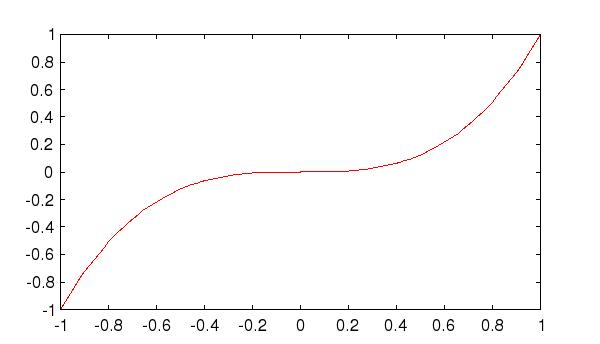
\includegraphics[width=8cm]{polyval1}}

